\documentclass[12pt]{article}

\usepackage{amsmath,amssymb,amsfonts} %In case we need math stuff
\usepackage{graphicx} %For inserting images and stuff
\usepackage{listings} %For inserting code snippets
\usepackage{enumerate} %For fancy enumeration
\usepackage{pdfpages} %For adding .pdf files
\usepackage{float} %Place diagrams at exactly where they are at in Latex code

\usepackage[margin=2cm]{geometry} %Nice margin setting

\title{ECSE 321 - Intro to Software Engineering\\Detailed Design}
\author{Harley Wiltzer\\Camilo Garcia La Rotta\\Jake Shnaidman\\Robert Attard\\Matthew Lesko}
\date{February 24, 2017}

\begin{document}
\pagenumbering{gobble} %No page number on title page
\maketitle
\newpage
\pagenumbering{arabic} %Arabic numeral page numbers on regular pages
\tableofcontents
\section{Description}
\subsection{Detailed Domain Model}
The Detail Design Diagram consists of the following entities: ApplicationManager, ProfileManager, CourseManager, Application, Profile, Course, Job, Instructor, Admin, Student, Laboratory, and Tutorial. It consists of a Controller, called Controller, a Boundary, called View, and a Persistence, called Persistence XStream. The Controller uses the entities ApplicationManager, ProfileManager, and CourseManager to save, edit, and modify data within the model, which are then saved within a persistence layer. The functionalities of the three "Manager" classes are listed below.
\begin{itemize}
	\item ApplicationManager is in charge of Application, the job application created and submitted by the student for a job. It is associated with Application, Job, and ProfileManager.
	\item ProfileManager creates Admin, Instructor, and Student entities, all of which inherit from the Profile class.
	\item CourseManager creates Course entities.
\end{itemize}
In total there will be three controller classes in the Controller Packages with an additional class for input exceptions or input validation. The three controller classes will each use at least one of the manager classes.
\subsection{Controller Packages}
There are two controller packages: one for the Desktop (Java) and Mobile (Android) platforms, and one for the Web (PHP) platform. The diagrams under Class Diagrams contain details on the controller classes' attributes and behavior for their respective package. These details include the attributes' names and types and the methods' signatures.
\subsection{View Packages}
There are three view packages: one for the Desktop (Java) platform, one for the Mobile (Android) platform, and one for the Web (PHP) platform. The diagrams under Class Diagrams contain details on the view classes' attributes and behavior for their respective package. These details include the attributes' names and types and the methods' signatures.
\section{Rationale}
\subsection{Detailed Domain Model}
The three Manager classes were needed in order to give functionality to the user to create the entities associated with the manager classes, except for ApplicationManager creating a ProfileManager. Having a separate controller for each manager class allows one to modify the functionality of one controller class with its respective manager class without it having to affect the other controller classes.
\section{Class Diagrams}
\subsection{Detailed Domain Model Diagram}
\begin{figure}[H]
	\centering
	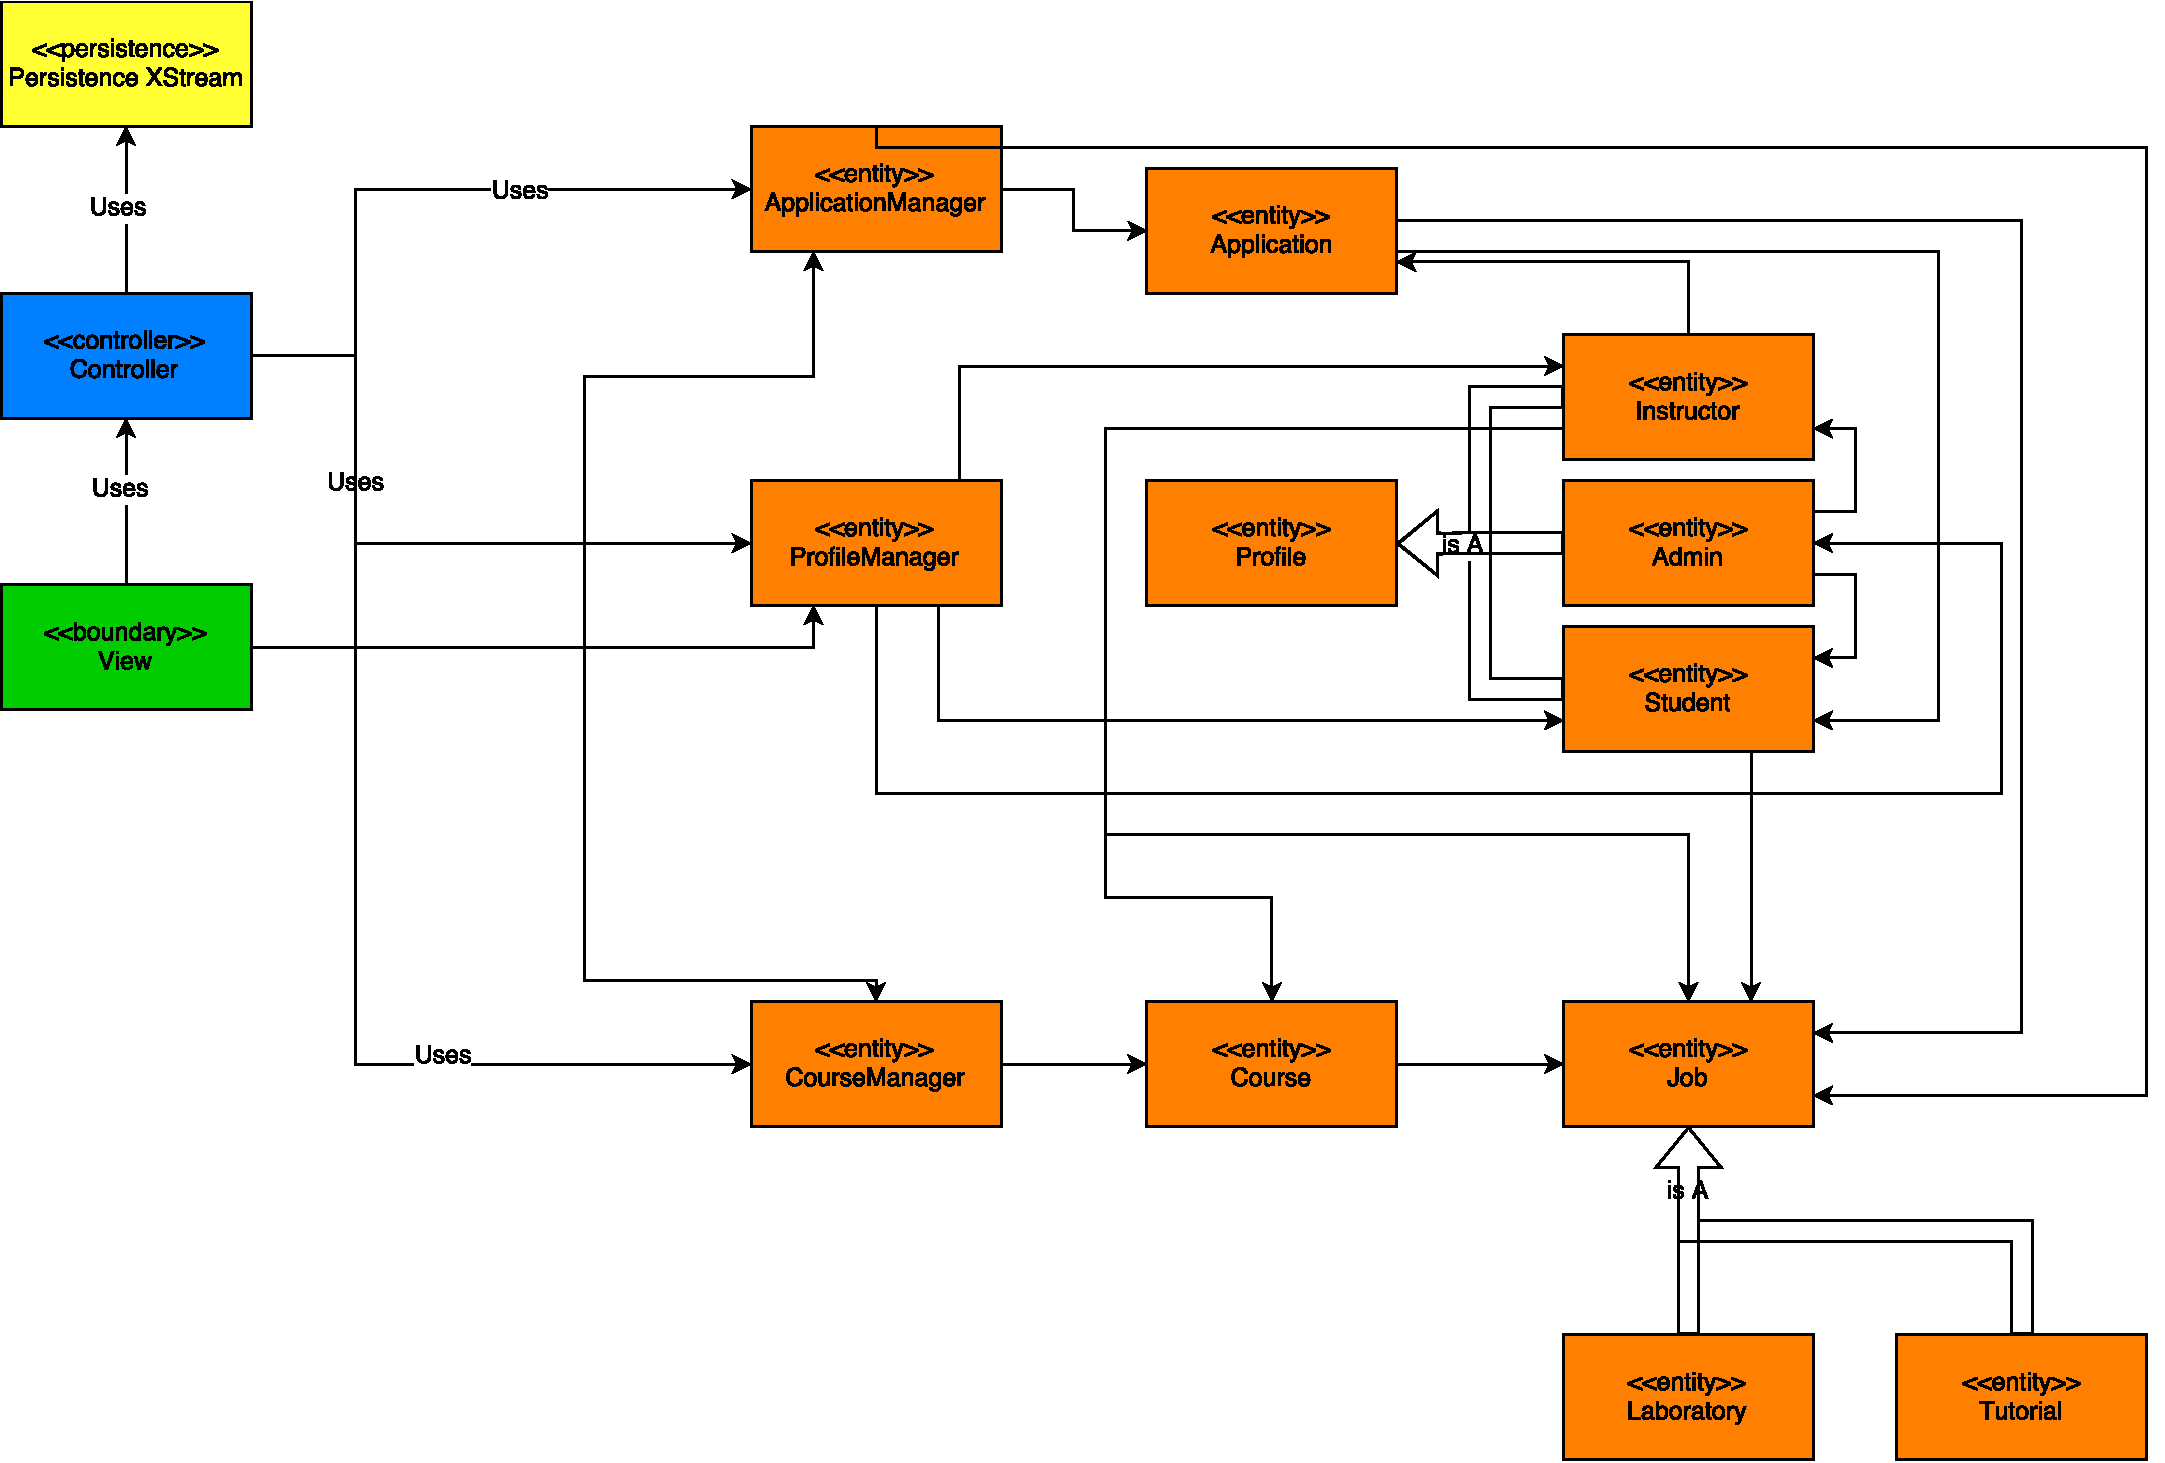
\includegraphics[width =1\textwidth]{./ClassDiagrams/DetailedDomainModelDiagram.pdf}
\end{figure}
\subsection{Java and Android Controller Class Diagram (Desktop and Mobile)}
\begin{figure}[H]
	\centering
	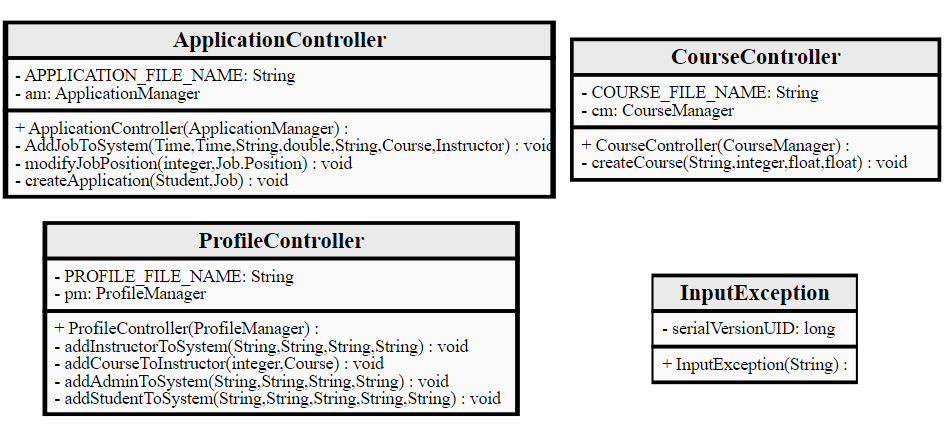
\includegraphics[scale=0.95]{./ClassDiagrams/ControllerPackageClassDiagramJava.png}
\end{figure}
\subsection{PHP Controller Class Diagram (Web)}
\begin{figure}[H]
	\centering
	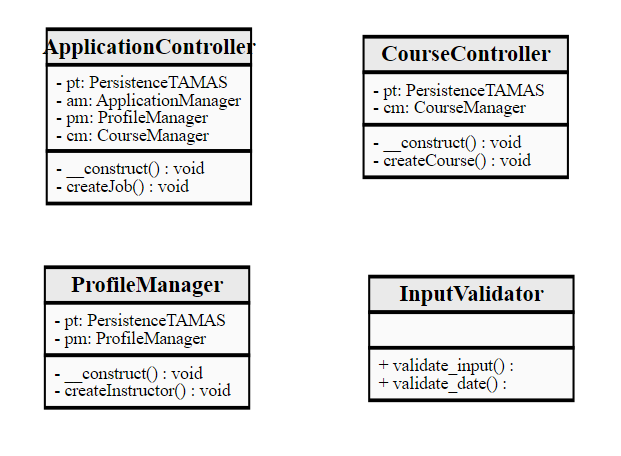
\includegraphics[scale=1.05]{./ClassDiagrams/ControllerPackageClassDiagramPHP.png}
\end{figure}
\subsection{Java View Class Diagram (Desktop)}
\begin{figure}[H]
	\centering
	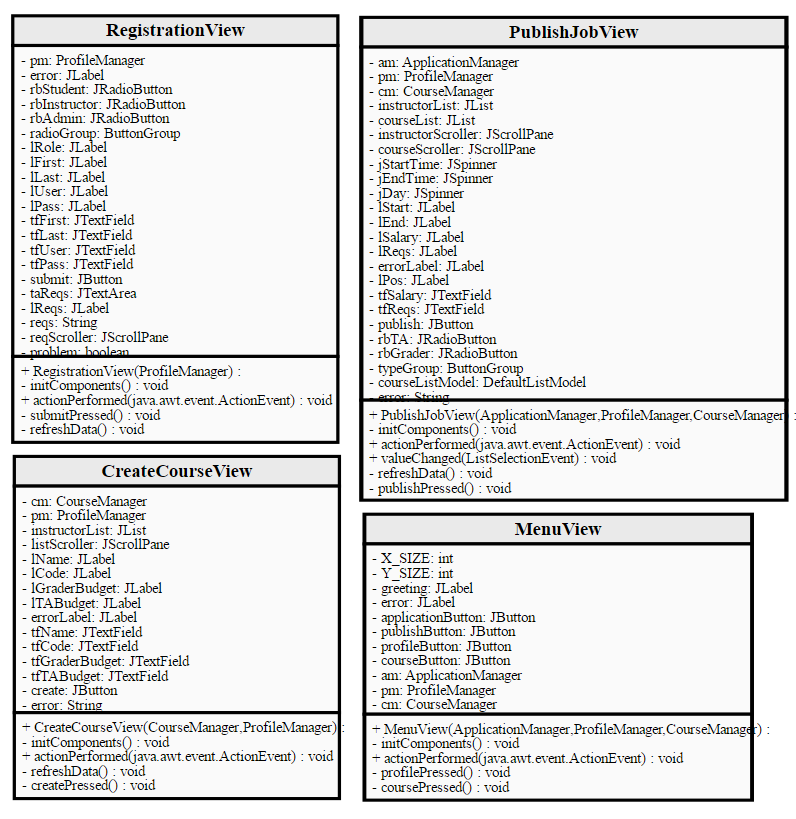
\includegraphics[scale=1]{./ClassDiagrams/desktopViewPackageDiagram(A).png}
	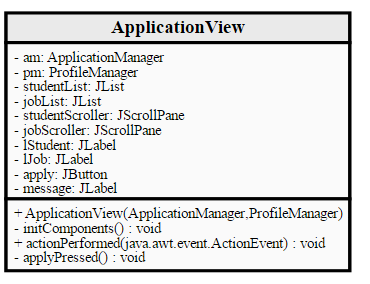
\includegraphics[scale=1]{./ClassDiagrams/desktopViewPackageDiagram(B).png}
\end{figure}
\subsection{PHP View Class Diagram (Web)}
\begin{figure}[H]
	\centering
	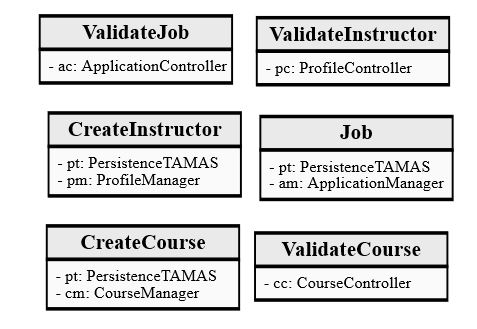
\includegraphics[]{./ClassDiagrams/WebViewPackageDiagram.jpg}
\end{figure}
\subsection{Android View Class Diagram (Android)}
%\begin{figure}[H]
%	\centering
%	\includegraphics[]{}
%\end{figure}
\end{document}
